\documentclass[12pt,a4paper]{article}
\usepackage[utf8]{inputenc} 
\usepackage[ngerman]{babel}
\usepackage[T1]{fontenc}
\usepackage{amsmath}
\usepackage{amsfonts}
\usepackage{amssymb}
\usepackage{graphicx}
\usepackage[left=2cm,right=2cm,top=2cm,bottom=2cm]{geometry}
\usepackage{physics}

\begin{document}
\section*{Young-Tableaus}


\begin{tabular}{cc}

\parbox{0.6\linewidth}{
 \textbf{Permutation} $P$: \\
\glqq Anordnung\grqq{}, spez. Reihenfolge von Elementen  \\
z.B. Operator 
$\hat{P} 
= \begin{pmatrix} a_1 & a_2 & a_3 \\ a_2 & a_3 & a_1 \end{pmatrix} \equiv \underbrace{
\begin{pmatrix} 1 & 2 & 3 \\ 2 & 3 & 1 \end{pmatrix}
}_{
\substack{\text{Reihenfolge} \\ \text{der Spalten} \\ \text{egal}}
}
\begin{array}{c}
  \\ \\ = \\ \\ \xleftarrow{\vspace{3cm}} \\
\end{array}
 \underbrace{
\begin{pmatrix} 1 & 2 & 3\end{pmatrix}
}_{\substack{\text{repräsentierbar}\\ \text{durch} \\ \text{Zyklus}} }$ \\ \\



$\hat{P}
= \begin{pmatrix} a_1 & a_2 & a_3 \\ a_2 & a_3 & a_1 \end{pmatrix} \equiv 
\begin{pmatrix} 1 & 2 & 3 \\ 2 & 3 & 1 \end{pmatrix}
= 
\begin{pmatrix} 1 & 2 & 3\end{pmatrix}
$ 
\\ \\

- permutiert Sequenz $a_1 a_2 a_3$ zu $a_2 a_3 a_1$ \\
- Anwendung auf z.B. 1: $(1 2 3)1 = 2$ \\
- Zyklusrepräsentation $\leftrightarrow$ Reihenfolge der Spalten egal
} 

 &
\parbox{0.6\linewidth}{
\textbf{Permutationsgruppe} $S_n$: \\
= $n!$ versch. Permutationen des Sets von $n$ Symbolen
} \\ \\

\parbox{0.6\linewidth}{
Permutation endlichen Sets = Produkt von Zyklen (ungleicher Elemente):\\
$P_c = P_a P_b$, wobei $P_b$ vor $P_a$ angewandt wird  \\
$\leftrightarrow$ \textbf{Transposition}: Zyklus mit 2 Symbolen


Zyklen ohne gleiche Elemente kommutieren, bei Element in beiden Zyklen nicht
} 

\\
\end{tabular}



$$  A =  \sum _Q (-1)^q Q$$



$$ S = \sum _P P$$










\begin{tabular}{p{4cm}|p{4cm}|p{4cm}|p{4cm}}
\centering [3] & \multicolumn{2}{p{8cm}|}{\centering [21]} &  \parbox[valign=c]{4cm}{ \centering [$1^3$]} \\ \hline  & & & \\
\centering 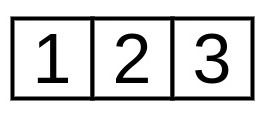
\includegraphics[scale=0.6]{build/young-123.jpg} & 
\parbox[valign=c]{4cm}{\centering 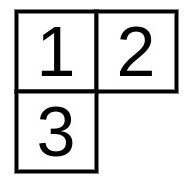
\includegraphics[scale=0.6]{build/young-12.jpg}}
& \parbox[valign=c]{4cm}{\centering 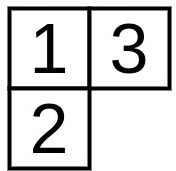
\includegraphics[scale=0.6]{build/young-13.jpg}}
& \parbox[valign=c]{4cm}{\centering 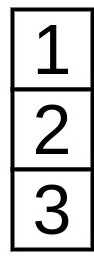
\includegraphics[scale=0.6]{build/young-3unten.jpg}}
\\ & & & \\ \hline 
$A$ fällt weg & $S$ bzgl. Indizes 1 und 2; $A$ bzgl. Indizes 1 und 3 & 
$S$ bzgl. Indizes 1 und 3; $A$ bzgl. Indizes 1 und 2 
& 
$S$ fällt weg \\ \hline
%$f^{(3)}_S $ 
%$= Y a_a b_2 c_3 = Sa_a b_2 c_3 $ 
%$= \sum _P P a_a b_2 c_3 
%= a_1b_2c_3 + a_1 b_3 c_2 + a_2 b_1 c_3 
%+ a_2 b_3 c_1 + a_3b_1c_2 + a_3 b_2 c_1
%$
%& 
%$f^{(3)}_1 = A \left( S a_1 b_2 c_3 \right) = A \left( 
%a_1 b_2 c_3 + a_2 b_1 c_3 \right) 
%$ 
%$ = a_1 b_2 c_3 - a_3 b_2 c_1 + a_2 b_1 c_3 - a_2b_3c_1$
%& 
%$f_2 ^{(3)} = A\left( S a_2 b_2 c_3\right) 
%= A\left( a_1 b_2 c_3 + a_3 b_2 c_1\right)
%= a_1 b_2 c_3 - a_2 b_1 c_3 + a_3 b_2 c_1 - a_3 b_1 c_2
%$
%&
%$f^{(3)}_A $ $= Y a_1 b_2 c_3 = A a_a b_2 c_3$ $\sum_Q (-1)^q Q a_1 b_2 c_3$ 
%$= a_1 b_2 c_3 - a_1 b_3 c_2 - a_2 b_1 c_3 + a_2 b_3 c_1 + a_3 b_1 c_2 - a_3 b_2 c_1$ 
%$= 
%\begin{vmatrix} a_1 & b_1 & c_1 \\ a_2 & b_2 & c_2 \\ a_3 & b_3 & c_3 \end{vmatrix}$ \\ \\
$f^{(3)}_S $ 
& 
$f^{(3)}_1 $
& 
$f_2 ^{(3)} $
&
$f^{(3)}_A $ \\ 
$= Y a_1 b_2 c_3 = Sa_1 b_2 c_3 $ 
& 
$ A \left( S a_1 b_2 c_3 \right) $
& 
$ = A\left( S a_1 b_2 c_3\right) 
$
&
$= Y a_1 b_2 c_3 = A a_1 b_2 c_3$ \\

$= \sum _P P a_1 b_2 c_3 
$
& 
$= A \left( 
a_1 b_2 c_3 + a_2 b_1 c_3 \right) $
& 
$= A\left( a_1 b_2 c_3 + a_3 b_2 c_1\right)
$
&
$=\sum_Q (-1)^q Q a_1 b_2 c_3$  \\
$
= a_1b_2c_3 + a_1 b_3 c_2 + a_2 b_1 c_3 
+ a_2 b_3 c_1 + a_3b_1c_2 + a_3 b_2 c_1
$
& 
$ = a_1 b_2 c_3 - a_3 b_2 c_1 + a_2 b_1 c_3 - a_2b_3c_1$
& 
$
= a_1 b_2 c_3 - a_2 b_1 c_3 + a_3 b_2 c_1 - a_3 b_1 c_2
$
&
$= a_1 b_2 c_3 - a_1 b_3 c_2 - a_2 b_1 c_3 + a_2 b_3 c_1 + a_3 b_1 c_2 - a_3 b_2 c_1$ \\
& & & $= 
\begin{vmatrix} a_1 & b_1 & c_1 \\ a_2 & b_2 & c_2 \\ a_3 & b_3 & c_3 \end{vmatrix}$ \\ \hline 
\end{tabular}

\vspace{1cm}




\newpage 
$ \ket{\frac{3}{2}\quad \frac{3}{2}}$ \\

$ \ket{\frac{3}{2}\quad \frac{1}{2}}$ \\

$ \ket{\frac{3}{2} \quad -\frac{1}{2}}$ \\

$ \ket{\frac{3}{2} \quad -\frac{3}{2}}$ \\

$ \ket{\frac{1}{2} \quad\frac{1}{2}}$ \\

$ \ket{\frac{1}{2} \quad-\frac{1}{2}}$ \\






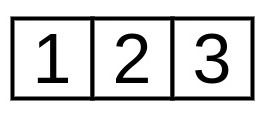
\includegraphics[scale=0.6]{build/young-123.jpg} : \\

$ \ket{\frac{3}{2}\quad \frac{3}{2}}$ \\

$ \ket{\frac{3}{2}\quad \frac{1}{2}}$ \\

$ \ket{\frac{3}{2} \quad -\frac{1}{2}}$ \\

$ \ket{\frac{3}{2} \quad -\frac{3}{2}}$ \\

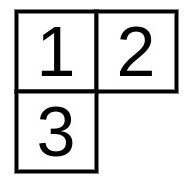
\includegraphics[scale=0.6]{build/young-12.jpg} : \\

$ \ket{\frac{1}{2} \quad\frac{1}{2}}$ \\

$ \ket{\frac{1}{2} \quad-\frac{1}{2}}$ \\

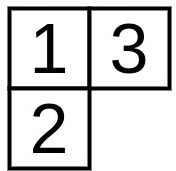
\includegraphics[scale=0.6]{build/young-13.jpg} : \\

$ \ket{\frac{1}{2} \quad\frac{1}{2}}$ \\

$ \ket{\frac{1}{2} \quad-\frac{1}{2}}$ \\



\newpage
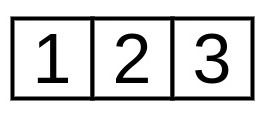
\includegraphics[scale=0.6]{build/young-123.jpg} : \\

$ \ket{\frac{3}{2}\quad \underbrace{\frac{3}{2}}_{\begin{array}{c}
\text{nur} \\ \text{Spin-up}
\end{array}}} = (\alpha \alpha \alpha )$ \\

$ \ket{\frac{3}{2}\quad \underbrace{\frac{1}{2}}_{\begin{array}{c}
1\;\alpha \text{-Spin im}  \\ \text{Überschuss}
\end{array} }} = \frac{1}{\sqrt{3}} \left[
 \left( \alpha \alpha \beta \right) +  \left( \beta \alpha \alpha \right) +  
 \left(    \alpha\beta \alpha \right) 
  \right]$ \\
  
$ \ket{\frac{3}{2}\quad \underbrace{-\frac{1}{2}}_{\begin{array}{c}
1\;\beta \text{-Spin im}  \\ \text{Überschuss}
\end{array} }} = \frac{1}{\sqrt{3}} \left[
 \left(\beta\beta \alpha \right) +  \left(  \alpha\beta \beta\right) +  
 \left(    \beta \alpha \beta\right) 
  \right]$ \\

$ \ket{\frac{3}{2}\quad \underbrace{-\frac{3}{2}}_{\begin{array}{c}
\text{nur} \\ \text{Spin-down}
\end{array}}} = (\beta \beta \beta )$ \\

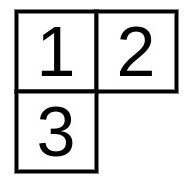
\includegraphics[scale=0.6]{build/young-12.jpg} : \\

$ \ket{\frac{1}{2} \quad\frac{1}{2}} = \frac{1}{\sqrt{2}} \left[ \left(\alpha\alpha \beta \right) - \left( \beta \alpha \alpha \right) \right]$ \\

$ \ket{\frac{1}{2} \quad-\frac{1}{2}}= \frac{1}{\sqrt{2}} \left[ \left( \alpha\beta \beta\right) - \left( \beta \alpha \beta\right) \right]$ \\

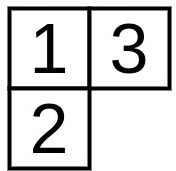
\includegraphics[scale=0.6]{build/young-13.jpg} : \\

$ \ket{\frac{1}{2} \quad\frac{1}{2}}= \frac{1}{\sqrt{2}} \left[ \left( \alpha \beta \alpha\right) - \left(\beta\alpha\alpha \right) \right]$  \\

$ \ket{\frac{1}{2} \quad-\frac{1}{2}}= \frac{1}{\sqrt{2}} \left[ \left( \alpha\beta\beta \right) - \left( \beta\alpha \beta\right) \right]$  \\ \\



$$\Psi = \ket{L S M_L M_S} \equiv \ket{{}^{2S+1}L M_L M_S} $$



\newpage

$ \ket{2 \quad 2}$ \\

$ \ket{2 \quad 1}$ \\

$ \ket{2 \quad 0}$ \\

$ \ket{2 \quad -1}$ \\

$ \ket{2 \quad -2}$ \\

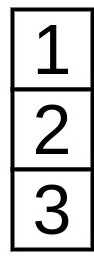
\includegraphics[scale=0.6]{build/young-3unten.jpg} : \\
$\ket{ 3\quad  M_L} $ mit $M_L \in \{-3, -2, -1, 0, 1, 2, 3\}$\\

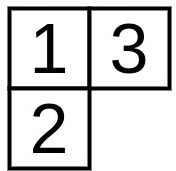
\includegraphics[scale=0.6]{build/young-13.jpg} : \\
$\ket{ 2\quad  M_L} $ mit $M_L \in \{-2, -1, 0, 1, 2\}$,\\
$\ket{ 1\quad  M_L} $ mit $M_L \in \{-1, 0, 1\}$\\

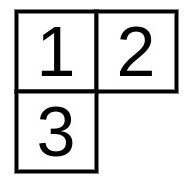
\includegraphics[scale=0.6]{build/young-12.jpg} : \\
$\ket{ 2\quad  M_L} $ mit $M_L \in \{-2, -1, 0, 1, 2\}$,\\
$\ket{ 1\quad  M_L} $ mit $M_L \in \{-1, 0, 1\}$\\


$$ \left( 1\quad 1 \quad 0\right) = p_{+1}(1) p_{+1}(2) p_{0}(3)$$


$$\ket{ 
\underbrace{
\underbrace{p}_{je\;in\;p\;Orbital}{}^{\overbrace{3}^{3\;Elektronen}} 
}_{Elektronenkonfiguration}
\quad 
\underbrace{{}^{\overbrace{2}^{2S + 1 \Leftrightarrow S = \frac{1}{2}}}\underbrace{D}_{L = 2} }_{Termsymbol}
\quad \underbrace{2}_{M_L} \quad 
\underbrace{\frac{1}{2}}_{M_S}
}$$

$$\Psi = \ket{p^{3} \quad{}^{2}D \quad 2 \quad\frac{1}{2}}
 = \sqrt{\frac{2}{3}} \left[ \ket{2\quad 2}_{II} \ket{\frac{1}{2} \quad\frac{1}{2}} - \ket{2\quad 2}_I \ket{\frac{1}{2}\quad\frac{1}{2}} \right]
$$





\end{document}